%!tex root=thesis.tex
\chapter{Machine Learning on Crowds}
\label{cha:ml}

\todo{Add a nice chapter summary.} In this chapter, I will introduce some
concepts from machine learning that I will use for the rest of this thesis. I
will discuss some common classification methods and techniques, image feature
extraction using convolutional neural networks, and methods to combat label noise.

\section{Classification}
\label{sec:classification}
    
    A common machine learning task, and indeed the machine learning focus of
    this thesis, is \emph{classification}. Given a set $\mathcal X$ of
    \emph{instances}, a set $\mathcal Y$ of \emph{labels}, the classification
    task is to assign a label $y \in \mathcal Y$ to each instance $x \in
    \mathcal X$. The ``true'' label of an instance is called the
    \emph{groundtruth}, and is denoted $z$. Classification thus amounts to
    modelling the conditional distribution $p(z \mid x)$. Some examples of
    classification include labelling images of digits, where $\mathcal X$ is a
    set of images and $\mathcal Y = \{0, \dots, 9\}$ \citep{lecun98}; and
    diagnosing breast cancer in patients, where $\mathcal X$ is a set of sets
    of medical observations and $\mathcal Y$ is the set $\{\text{malignant},
    \text{benign}\}$ \citep{wolberg90}.

    Modelling $p(z \mid x)$ requires some set of \emph{training data} $\mathcal
    D \subset \mathcal X \times \mathcal Y$. The training data are either used
    to find parameters for a model or to estimate the model directly. Both
    processes are called \emph{training} the model. The cardinality of the
    training data is denoted $N = |\mathcal D|$.

    \emph{Binary classification} is classification where each instance must be
    assigned one of two labels, i.e. $\mathcal Y \sim \{0, 1\}$. Instances with
    a true label of $0$ are called \emph{negative instances}, and instances
    with a true label of $1$ are called \emph{positive instances}. For this
    thesis, I will focus entirely on binary classification.

    Instances are usually represented by a vector of \emph{features}, denoted
    $\vec x$. Choosing features is an important and non-trivial part of
    modelling a classification task, and can strongly affect the ability of a
    model to classify instances. The dimensionality of the feature space is
    denoted $D$ and we assume that $\mathcal X = \mathbb{R}^D$.

    In this section, I will introduce two common ways of modelling binary
    classification: logistic regression, and random forests.

    \subsection{Logistic Regression}
    \label{sec:logistic-regression}

        Logistic regression is a simple linear model of binary classification.
        The conditional distribution $p(z \mid \vec x)$ is modelled as
        \[
            y(\vec x) = p(z = 1 \mid \vec x) = \sigma(\vec w^T \vec x + b),
        \]
        where $\vec w$ and $b$ are parameters to the model and $\sigma$ is the
        logistic sigmoid function
        \[
            \sigma(t) = \frac{1}{1 + \exp(-t)}.
        \]
        The elements of $\vec w$ are called the \emph{weights}, and control the
        effect of each feature on the output label probability. $b$ is the
        \emph{bias}, a constant added to all weighted sums of features
        independent of the features themselves. $b$ can be incorporated into
        $\vec w$ by adding an extra feature to $\vec x$ that is always $1$ and
        increasing the dimension of $\vec w$ by 1. I adopt this convention for
        the remainder of this thesis whenever $b$ is not explicitly included.

        Logistic regression is differentiable, and so may be trained using
        \emph{gradient descent}. In gradient descent, $\vec w$ is modified by
        the update equation
        \[
            \vec w \leftarrow \vec w - \lambda \nabla L(\vec w),
        \]
        where $L : \mathbb{R}^D \to \mathbb{R}$ is the \emph{loss} function and
        $\lambda \in (0, 1)$ is the \emph{learning rate}.

        The loss function represents how well the current model fits the
        observations. For binary classification, this is usually given by the
        \emph{cross-entropy error}
        \[
            L(\vec w) = -\frac{1}{N} \sum_{\vec x, z \in \mathcal D} \left(
                z \log y(\vec x) + (1 - z) \log (1 - y(\vec x))
            \right)
        \]
        with gradient
        \[
            \nabla L(\vec w) = -\frac{1}{N}
                \sum_{\vec x, z \in \mathcal D} \left(z - y(\vec x)\right).
        \]

    \subsection{Random Forests}
    \label{sec:random-forests}

        \todo{Write this section.}

\section{Feature Extraction from Images}
\label{sec:image-features}
    
    For instances to be input to a classification model, they must be
    represented by vectors of features. Feature selection is generally a hard
    problem, but it may be straightforward if instances are simple vectors of
    measurements (such as in the breast cancer dataset described in Section
    \ref{sec:breast-dataset}). If the instances are provided in the form of
    images, however, feature selection becomes considerably harder.

    \subsection{The Na\"ive Approach}
    \label{sec:naive-approach-image-features}

        Images can be thought of as vectors of pixels, where the value of each
        pixel is treated as an independent feature. If the image is a colour
        image, then each channel (red, blue, and green) of each pixel can be
        treated as an independent feature. This is a very simple way to obtain
        features from images, with two considerable problems.

        The first problem with this approach is that images tend to be large.
        Taking each pixel as a feature leads to high dimensional feature spaces.
        This is not ideal as many algorithms perform poorly in high dimensional
        spaces. This can be resolved using \emph{pooling}, which we describe in
        Section \ref{sec:pooling}.

        The second problem is that using pixels directly as independent features
        fails to accurately capture the image. The pixels are assumed
        independent when this is not the case --- neighbouring pixels are likely
        to be correlated, shapes and structure within the image introduce
        further correlations, and so on. If we are only looking at certain kinds
        of images, then the pixel location may also matter --- for example, we
        might have as inputs photographs of landscapes, where the sky tends to
        be at the top of the image --- and this information is also lost. These
        effects are shown in Figure \ref{fig:shuffled-face}. In Section
        \ref{sec:convolutions}, we describe a common approach for resolving this
        problem.

        \begin{figure}[!ht]
            \centering
            \begin{subfigure}[t]{0.5\textwidth}
                \centering
                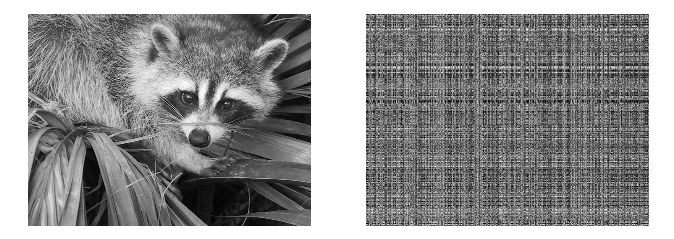
\includegraphics[width=\textwidth]{images/face.png}
            \end{subfigure}%
            ~
            \begin{subfigure}[t]{0.5\textwidth}
                \centering
                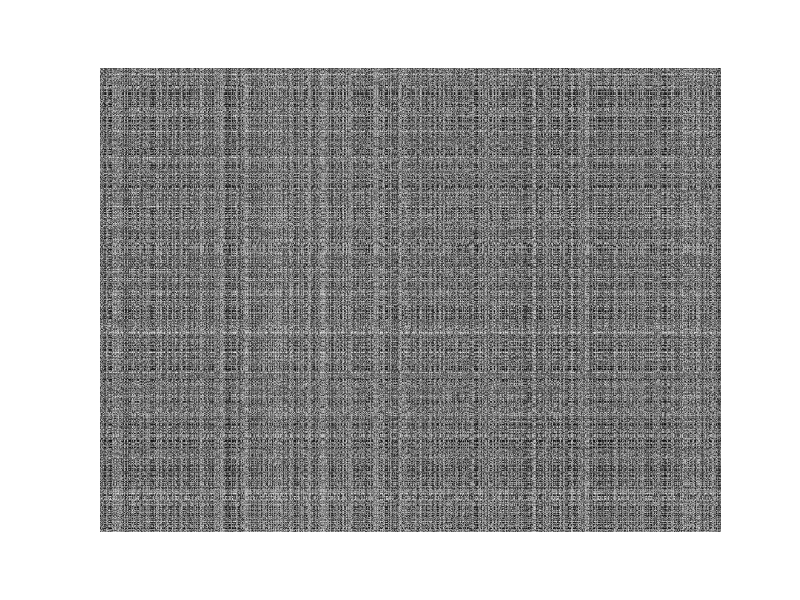
\includegraphics[width=\textwidth]{images/face_shuffled.png}
            \end{subfigure}
            \caption{If we ignore the location of pixels when interpreting an
                image as a vector, these two images have identical feature
                vectors, despite the left image clearly containing information
                not present in the right image.}
            \label{fig:shuffled-face}
        \end{figure}

    \subsection{Pooling}
    \label{sec:pooling}

        Pooling is a class of operations that reduce the dimensionality of an
        image, parameterised by a \emph{pool size} $p$\footnote{Another
        parameter is the \emph{stride} $s$, which we ignore here for simplicity,
        setting $s = p$.}. Nonoverlapping $p \times p$ squares of pixels are
        condensed into one value, which becomes the corresponding pixel in the
        output. In this way, the size of the image is reduced from $m \times n$
        to $\frac{m}{p} \times \frac{n}{p}$. We are free to choose whatever
        aggregation operation we like to condense squares of pixels; common
        choices are $\max$ (called \emph{max pooling}) and $\mbox{mean}$ (called
        \emph{average pooling}). Some pooling examples are shown in Figure
        \ref{fig:pooling}.
        
        \begin{figure}[!ht]
            \centering
            \begin{subfigure}[t]{0.5\textwidth}
                \centering
                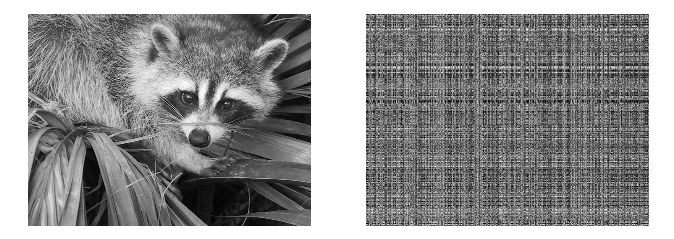
\includegraphics[width=\textwidth]{images/face.png}
                \caption{Original image.}
                \label{fig:pooling-face-original}
            \end{subfigure}%
            ~
            \begin{subfigure}[t]{0.5\textwidth}
                \centering
                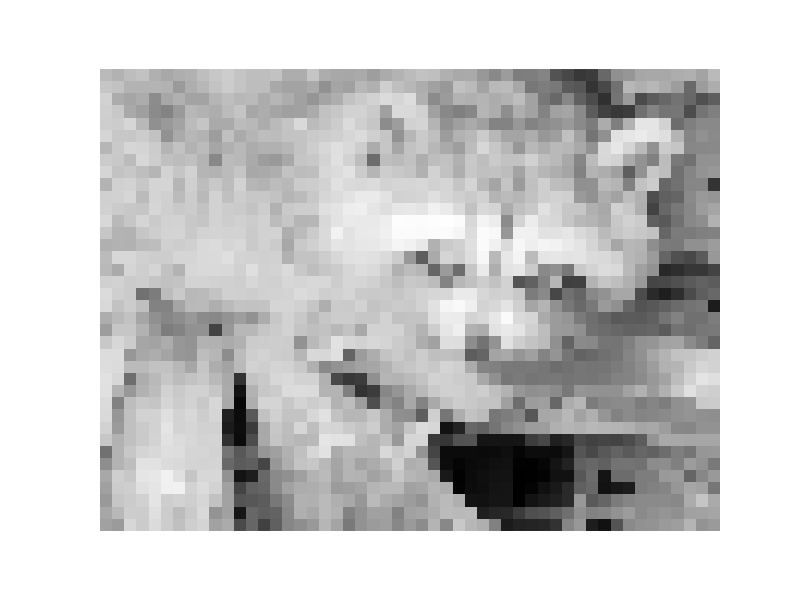
\includegraphics[width=\textwidth]{images/face_max_pooled.png}
                \caption{Max pooling.}
                \label{fig:pooling-face-max}
            \end{subfigure}
            \begin{subfigure}[t]{0.5\textwidth}
                \centering
                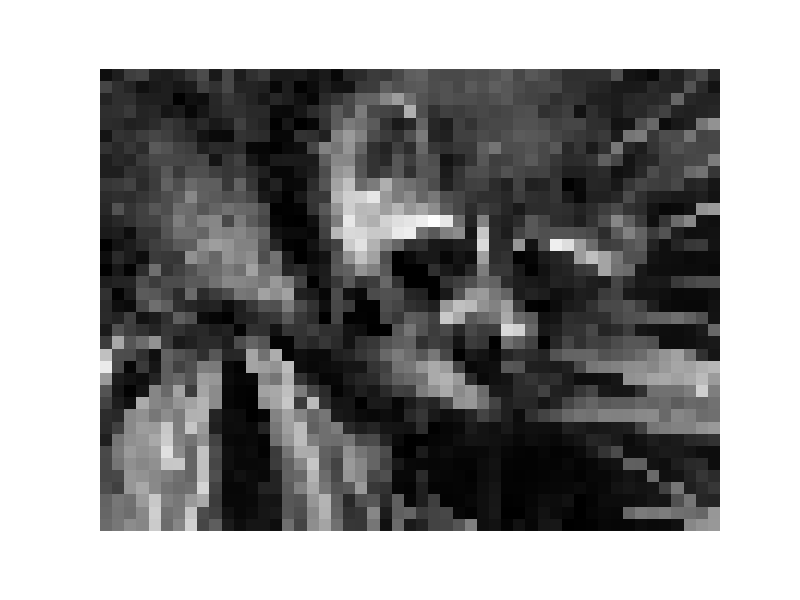
\includegraphics[width=\textwidth]{images/face_min_pooled.png}
                \caption{Min pooling.}
                \label{fig:pooling-face-min}
            \end{subfigure}%
            ~
            \begin{subfigure}[t]{0.5\textwidth}
                \centering
                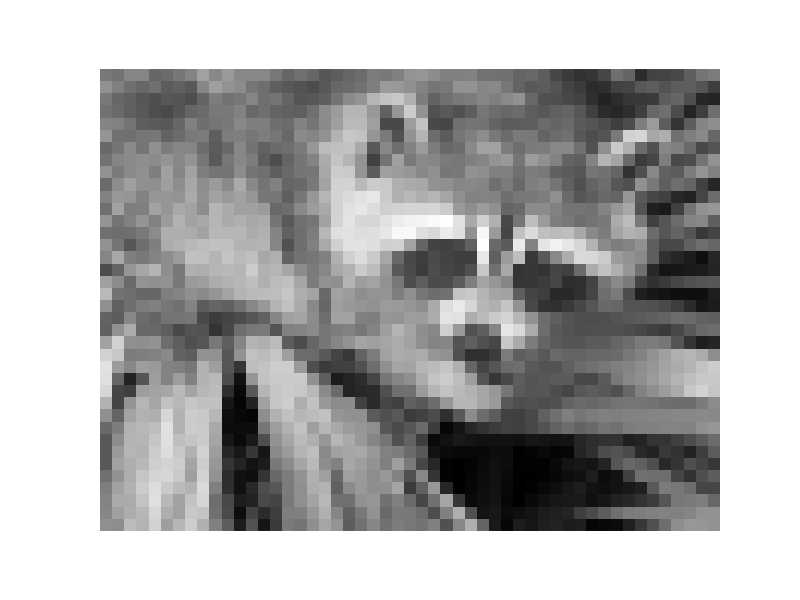
\includegraphics[width=\textwidth]{images/face_average_pooled.png}
                \caption{Average pooling.}
                \label{fig:pooling-face-average}
            \end{subfigure}%
            \caption{Examples of max, min, and average pooling applied to an
                image.}
            \label{fig:pooling}
        \end{figure}

    \subsection{Convolutions}
    \label{sec:convolutions}

        \begin{figure}[!ht]
            \centering
            \begin{subfigure}[t]{0.5\textwidth}
                \centering
                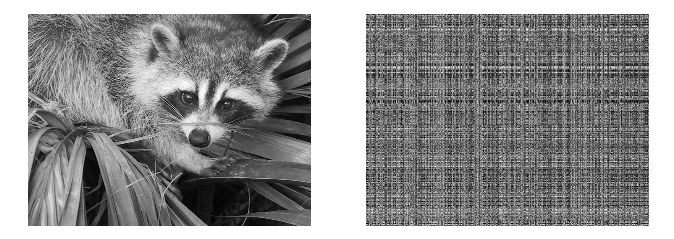
\includegraphics[width=\textwidth]{images/face.png}
                \caption{Original image.}
                \label{fig:convolution-face-original}
            \end{subfigure}%
            ~
            \begin{subfigure}[t]{0.5\textwidth}
                \centering
                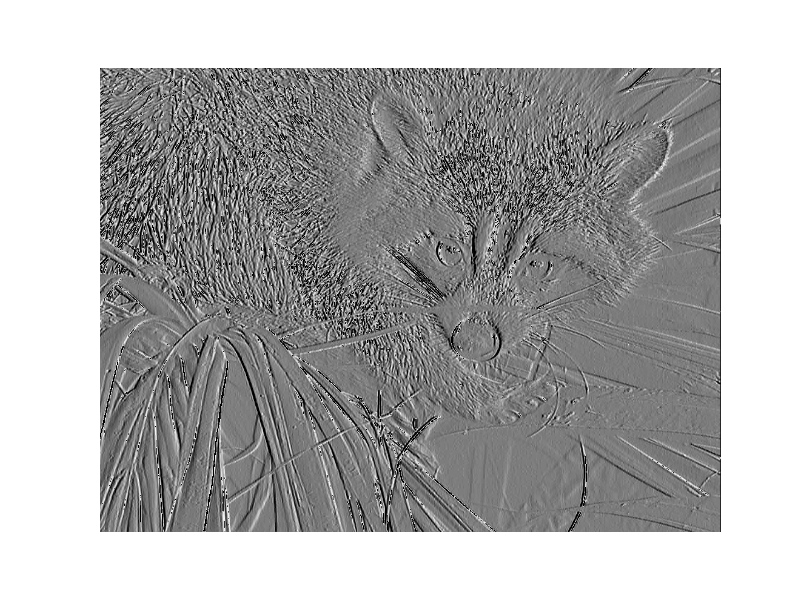
\includegraphics[width=\textwidth]{images/face_convolved.png}
                \caption{Convolved image.}
                \label{fig:convolution-face-convolved}
            \end{subfigure}
            %
            \begin{subfigure}[t]{0.3\textwidth}
                \centering
                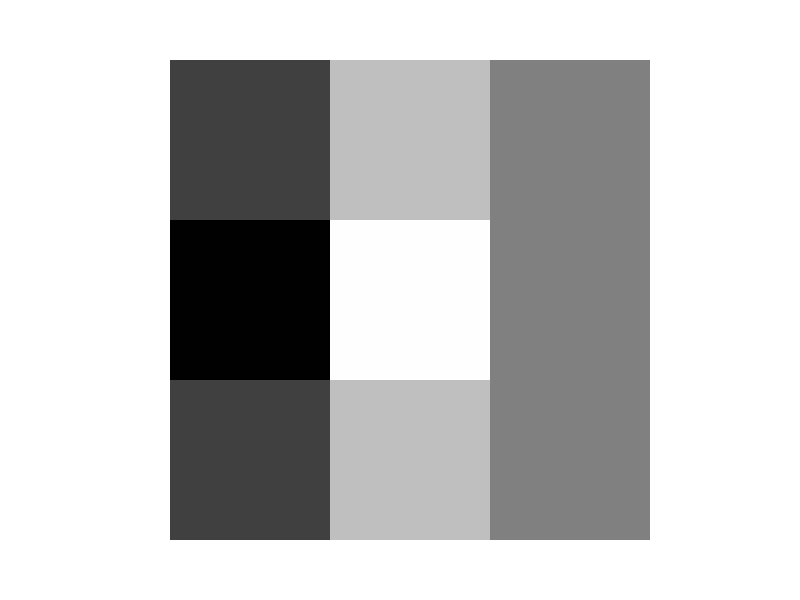
\includegraphics[width=\textwidth]
                    {images/convolutional_filter.png}
                \caption{Convolutional filter.}
                \label{fig:convolution-face-filter}
            \end{subfigure}
            \caption{Convolving an image with a $3 \times 3$ filter gives a new
                image. This filter acts as a kind of vertical edge detector.}
            \label{fig:convolved-face}
        \end{figure}

        A common way to make use of neighbourhood information in images is by
        using \emph{convolutions}. A convolution is an operation that transforms
        an image by applying an $n \times n$ \emph{filter} to each $n \times n$
        square of pixels. The filter is a matrix in $\mathbb{C}^{n \times n}$,
        and it is applied to a square of pixels by treating that square as a
        matrix, performing an elementwise multiplication between the filter
        matrix and the pixel matrix, and summing the result. Applying the filter
        to a square of pixels gives a single pixel value, so by applying the
        filter across the image, a new image is generated \citep{ludwig15}.

        One ambiguity here is how to apply a filter to the edges of an image.
        There are multiple possible ways to do this. The most common method is
        to only apply the filter to squares of pixels fully contained within the
        image, making the output image smaller than the input. Another method is
        to apply the filter to the edges and assume that pixels outside the
        image have a constant value (usually 0), making the output image the
        same size as the input. These methods are commonly known as ``valid''
        and ``same'' respectively in libraries such as SciPy and Keras.

        The effect of a simple convolutional filter on an image is shown in
        Figure \ref{fig:convolved-face}, and an algorithm for performing a
        convolution is shown in Algorithm \ref{alg:convolution}.

        \begin{algorithm}[!ht]
            \KwData{\\\quad{}An image $X \in \mathbb{R}^{m \times n}$%
                    \\\quad{}A filter $F \in \mathbb{C}^{d \times d}$}
            \KwResult{An image $\in \mathbb{R}^{(m - d + d \text{ mod } 2) \times (n - d + d \text{ mod } 2)}$}

            Initialise output image $Y \in \mathbb{R}^{(m - d + d \text{ mod } 2) \times (n - d + d \text{ mod } 2)}$\;
            \For{$y \in \lfloor d/2 \rfloor, \dots, m - \lfloor d/2 \rfloor$}{
                \For{$x \in \lfloor d/2 \rfloor, \dots, n - \lfloor d/2 \rfloor$}{
                    $H \leftarrow$ $d \times d$ square of pixels centred on $(x, y)$\;
                    $Y_{y, x} \leftarrow (\vec 1^T (H \odot F) \vec 1) / (\vec 1^T F \vec 1)$\;
                }
            }

            \KwRet{$Y$}
            \caption{One method of performing a convolution. Here, we choose to
                use the ``valid'' method of handling edges, resulting in a
                smaller output than the input. $\odot$ is the elementwise
                matrix product.}
            \label{alg:convolution}
        \end{algorithm}

        By repeatedly applying convolutions, we can extract features from images
        that would not have been present using the na\"ive approach of Section
        \ref{sec:naive-approach-image-features}.

\section{Crowdsourcing Labels}
\label{sec:crowdsourcing}

    For standard supervised learning tasks, the labels are generally
    provided by some \emph{expert}, carrying the assumption that these
    labels are correct and represent the groundtruth. More recently,
    however, many projects have \emph{crowdsourced} their labels: Non-expert
    people (the \emph{crowd}) volunteer or are paid to label data. The most
    obvious advantage of crowdsourcing is that crowds are able to cheaply or
    quickly label large amounts of data simply because there are so many
    people labelling. The crowd may be sourced from websites like Amazon
    Mechanical Turk\footnote{\url{http://mturk.com}} where small amounts of
    money are paid on a per-label basis, or they may volunteer out of
    interest in the labelling project.

    \subsection{Motivation}
    \label{sec:crowdsourcing-motivation}

        \todo{Write}

    \subsection{Examples}
    \label{sec:crowdsourcing-examples}

        Some notable examples of projects with crowdsourced labels include
        Galaxy Zoo \citep{lintott08}, a project to identify morphologies of
        galaxies from the Sloan Digital Sky Survey that has gathered tens of
        millions of labels for nearly 900 000 galaxies from over 80 000
        volunteers \citep{lintott11}; and Snapshot Serengeti \citep{swanson15},
        a project to observe mammals in Serengeti National Park that has
        classified nearly 11 million camera trap images with the help of 28 000
        volunteers.

        \todo{Rewrite and extend}

    \subsection{Problems}
    \label{sec:crowdsourcing-problems}

        Crowdsourcing is not without downsides. Since the crowd necessarily
        consists of non-experts, there is no longer any guarantee that labels
        are correct --- indeed, for the Radio Galaxy Zoo, balanced accuracy of
        individual labellers varies from 40--100\%, with an average of 71\%.
        Additionally, labels from different labellers may be correlated,
        different labellers may be better skilled at labelling different kinds
        of examples, some examples may be intrinsically hard for non-experts to
        label, and labellers may even be actively malicious in giving incorrect
        labels.

        \todo{Rewrite and extend}

\section{Simulating a Crowd Labelling Task}
\label{sec:crowd-simulation}
    
    In Section \ref{sec:crowd-labels}, we will discuss some ways of mitigating
    the problems with crowdsourced labels. To test these methods, we will need a
    reproducible way of obtaining crowd labels. Since the crowd is inherently
    unpredictable, we cannot use an existing crowd-labelled dataset for testing,
    so we must instead simulate a crowd labelling task based on a dataset with
    known groundtruth. In this section, we describe our method for simulating a
    crowd labelling task, which we then employ to test methods in Section
    \ref{sec:crowd-labels}.

    \subsection{The Breast Cancer Wisconsin Dataset}
    \label{sec:breast-dataset}

        The breast cancer Wisconsin dataset, first used by
        \citeauthor{wolberg90}, presents a classification task commonly used for
        testing classification methods. The dataset can be obtained from the UCI
        Machine Learning Repository \citep{lichman13}
        \footnote{\url{https://archive.ics.uci.edu/ml/%
                       datasets/Breast+Cancer+Wisconsin+\%28Original\%29}}.
        The classification task is, given medical observations of a patient,
        determine if their cancer is benign or malignant. Each instance is a
        10-dimensional feature vector, and there are 699 instances. There is
        some missing data, which we chose to set to 0.

    \subsection{Simulated Labeller Representation}
    \label{sec:simulated-labellers}

        We simulate $T$ labellers. Each labeller is indexed by a number $t$. The
        $t$th labeller is represented by their \emph{sensitivity} or \emph{true
        positive rate} $\alpha_t$, and their \emph{specificity} or \emph{true
        negative rate} $\beta_t$, i.e.
        \begin{align*}
            \alpha_t &= p(y_t = 1 \mid z = 1)\\
            \beta_t &= p(y_t = 0 \mid z = 0)
        \end{align*}
        where $y_t$ is the label assigned by the $t$th labeller to an instance
        with groundtruth $z$.

    \subsection{Obtaining the Simulated Labels}
    \label{sec:obtaining-simulated-labels}

        To generate crowd labels from our $T$ simulated labellers, we follow Algorithm \ref{alg:simulated-crowd}.

        \begin{algorithm}[H]
            \KwData{\\\quad{}A set of groundtruth labels $\{z_1, \dots, z_N\}$\\\quad{}A set of labellers $\{(\alpha_1, \beta_1), \dots, (\alpha_T, \beta_T)\}$.}
            \KwResult{A set of crowd labels $\{y_{1, 1}, \dots, y_{T, N}\}$.}

            \For{$i \in 1, \dots, N$}{
                \For{$t \in 1, \dots, T$}{
                    \eIf{$z_i = 1$}{
                        \WithProb{$\alpha_t$}{
                            $y_{t, i} \leftarrow 1$\;
                        }
                        \Else{
                            $y_{t, i} \leftarrow 0$\;
                        }
                    }{
                        \WithProb{$\beta_t$}{
                            $y_{t, i} \leftarrow 0$\;
                        }
                        \Else{
                            $y_{t, i} \leftarrow 1$\;
                        }
                    }
                }
            }
            \KwRet{$\{y_{1, 1}, \dots, y_{T, N}\}$}
            \caption{Simulating a crowd labelling task.}
            \label{alg:simulated-crowd}
        \end{algorithm}

\section{Aggregating Crowd Labels}
\label{sec:crowd-labels}

    \todo{Introduce}

    % There's kind of two things going on here - using multiple labels, and
    % using labels where the groundtruth doesn't exist. I should write about
    % that.

    In crowd learning scenarios, it is common to have multiple labels for a data
    point with no known groundtruth.

    \todo{extend}

    \subsection{Using Raw Labels}
    \label{sec:raw-labels}

        \todo{Write}

    \subsection{Majority Vote}
    \label{sec:majority-vote}

        One way to reduce label noise is to allow multiple labellers to label
        the same examples, and then for each example take the \emph{majority
        vote} to find a ``consensus'' label. If the label provided by the $t$th
        labeller is denoted $y_t$ and there are $T$ labellers, then the
        consensus label is given by
        \begin{equation*}
            y = \begin{cases}
                1 & \frac{1}{T} \sum_{t = 1}^T y_t > 0.5\\
                0 & \frac{1}{T} \sum_{t = 1}^T y_t < 0.5\\
            \end{cases}
        \end{equation*}
        with the remaining case decided evenly at random \citep{raykar10}.

        The idea is that the majority of labels are correct, so with
        sufficiently large amounts of relabelling we expect the label noise to
        be reduced. How large ``sufficiently large'' is is unclear and domain-
        dependent, and is outside the scope of this thesis, though papers like
        \citet{sheng08} and \citet{lin16} provide some information on how to
        choose relabelling rates. Of course, this fails in situations where the
        majority of labellers are not correct, which may be due to intrinsic
        difficulty or malicious labelling, or where there is no clear majority.

        \todo{Discuss weighted majority vote.}

    \subsection{Raykar et al. Model}
    \label{sec:raykar}

        One way to learn from crowdsourced labels when no groundtruth is
        available is to jointly model both the reliability of each labeller (the
        \emph{labeller model}) and the groundtruth itself (the
        \emph{classification model}).

        \citet{raykar10} proposed such a joint model, which we describe here.

        The accuracy of the $t$th labeller is modelled by the sensitivity
        $\alpha_t$ and the specificity $\beta_t$, as described in Section
        \ref{sec:simulated-labellers}. This model assumes that labeller
        reliability is independent of the example $x$, but dependent on the
        groundtruth label $z$. Note that under this model, the probability that
        labeller $t$ will assign a given label to a positive example is given by
        \begin{equation*}
            p(y_t \mid z = 1, \alpha_t) =
                (\alpha_t)^{y_t} (1 - \alpha_t)^{1 - y_t}
        \end{equation*}
        and the probability that they will assign a given label to a negative
        example is given by
        \begin{equation*}
            p(y_t \mid z = 0, \beta_t) =
                (\beta_t)^{1 - y_t} (1 - \beta_t)^{y_t}.
        \end{equation*}
        For ease of notation, let $\vec \alpha = (\alpha_1, \dots, \alpha_t)$
        and $\vec \beta = (\beta_1, \dots, \beta_t)$.

        With this method, the classification model can be any classifier.
        \citeauthor{raykar10} choose to use logistic regression:
        \begin{equation}
            \label{eq:raykar-logreg}
            p(z = 1 \mid \vec x, \vec w) = \sigma(\vec w^T \vec x).
        \end{equation}

        The model parameters $\vec \theta = \{\vec w, \vec \alpha, \vec \beta\}$
        can be found by maximising the likelihood. Under the assumption that
        examples are independently sampled and labellers are independent, the
        likelihood is given by
        \begin{align*}
            p(\mathcal D \mid \vec \theta) &=
                \prod_{i = 1}^N
                    \prod_{t = 1}^T
                        p(y_{t, i} \mid \vec x_i, \vec w, \alpha_t, \beta_t)\\
            &\begin{aligned}=
                \prod_{i = 1}^N
                    \prod_{t = 1}^T
                        &\bigg[p(y_{t, i} \mid z_i = 1, \alpha_t)
                            p(z_i = 1 \mid \vec x_i, \vec w)\\
                        &+ p(y_{t, i} \mid z_i = 0, \beta_t)
                            p(z_i = 0 \mid \vec x_i, \vec w)\bigg].
             \end{aligned}
        \end{align*}
        Since there are unknown values $z$, the maximum likelihood problem must
        be solved using expectation-maximisation. This has closed-form solutions
        for $\vec \alpha$ (Equation \ref{eq:raykar-alpha}) and $\vec \beta$
        (Equation \ref{eq:raykar-beta}), but gradient methods must be used for
        finding $\vec w$.

        $\mu_i$ is initialised with majority vote, i.e.
        \begin{equation*}
            \mu_i = \frac{1}{T} \sum_{t = 1}^T y_{t, i}.
        \end{equation*}
        The expectation step requires us to compute
        \begin{align*}
            a_i &= \prod_{t = 1}^T
                (\alpha_t)^{y_{t, i}} (1 - \alpha_t)^{1 - y_{t, i}}\\
            b_i &= \prod_{t = 1}^T
                (\beta_t)^{1 - y_{t, i}} (1 - \beta_t)^{y_{t, i}}\\
            \mu_i &\propto
                \frac{a_i \sigma(\vec w^T \vec x_i)}
                     {a_i \sigma(\vec w^T \vec x_i) +
                      b_i (1 - \sigma(\vec w^T \vec x_i))}.
        \end{align*}
        The maximisation step requires us to compute
        \begin{align}
            \label{eq:raykar-alpha}
            \alpha_t &= \frac{\sum_{i = 1}^N \mu_i y_{t, i}}
                             {\sum_{i = 1}^N \mu_i}\\
            \label{eq:raykar-beta}
            \beta_t &= \frac{\sum_{i = 1}^N (1 - \mu_i) (1 - y_{t, i})}
                            {\sum_{i = 1}^N (1 - \mu_i)}
        \end{align}
        and find the $\vec w$ that maximises the likelihood using gradient
        methods. In my implementation of this algorithm, I initialised $\vec w$
        using logistic regression trained on the majority vote, and then used
        the old $\vec w$ to initialise each subsequent maximisation step.

        As part of this thesis, I have produced an open source implementation of
        this algorithm, described in Section \ref{sec:crowdastro-raykar}. I then
        performed a series of experiments using this implementation, which I
        describe here.

        \subsubsection{Testing the Raykar Classifier}

            I first used the implementation to perform a simple, simulated crowd
            labelling problem. Five simulated labellers were assigned true positive
            and false positive rates uniformly distributed in the range $[0.25,
            0.75]$. Each simulated labeller labelled 50\% of the breast cancer dataset \todo{backref}. Random samples of
            75\% of the examples were drawn 20 times and used to train both the
            \citeauthor{raykar10} classifier and a logistic regression classifier
            (using majority vote for the labels). These classifiers were tested
            against the groundtruth of the remaining 25\%. The results are plotted
            in Figure \ref{fig:raykar}. The Raykar classifier attained a balanced
            accuracy of $(58 \pm 8)\%$ and the logistic regression classifier
            attained a balanced accuracy of $(56 \pm 8)\%$.

            \begin{figure}[!ht]
                \centering
                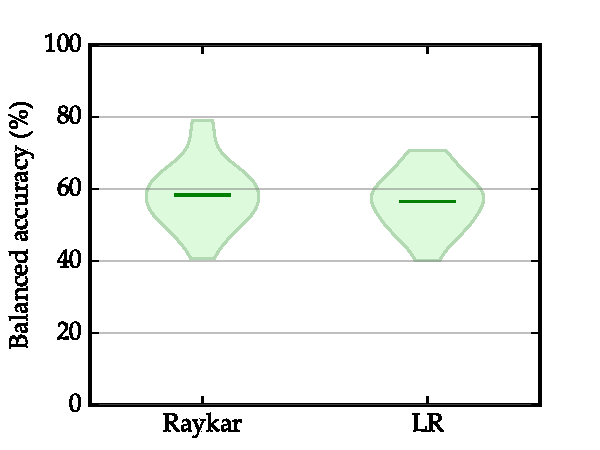
\includegraphics[width=\textwidth]{images/experiments/raykar.pdf}
                \caption{Performance of the \citeauthor{raykar10} classifier against
                    logistic regression on a simulated crowd labelling of the breast
                    cancer dataset \citep{wolberg90}.}
                \label{fig:raykar}
            \end{figure}

        \subsubsection{The Effect of Class Imbalance}

            The second experiment tested the effect of class imbalance on the
            resulting balanced accuracy of the classifier, as well as on the
            predicted $\alpha$ and $\beta$ for each labeller. Scikit-learn's \citep
            {scikit-learn} \texttt{sklearn.datasets.make\_classification} function
            was used to generate datasets with 5-dimensional features (of which 3
            were informative, and 2 were redundant) with a class separation of 1 and
            1\% of true labels randomly flipped. Five datasets were generated, with
            different ratios of negative to positive examples. The ratios were
            $4:1$, $2:1$, $1:1$, $1:2$, and $1:4$. 1000 examples were drawn for each
            dataset. A crowd labelling task was then simulated, assigning 10
            labellers true positive and false positive rates uniformly at random in
            the interval $[0.5, 0.9]$ and allowing them to ``label'' the examples.
            The same labellers were used across all trials and datasets. The
            \citeauthor{raykar10} algorithm was then run on each dataset and the
            balanced accuracy and output $\alpha$ and $\beta$ values were recorded
            for each. The experiment was repeated five times. The resulting balanced
            accuracies are plotted against the ratios of negative to positive
            examples in Figure \ref{fig:raykar-class-balance-ba}, and the estimated
            $\alpha$ and $\beta$ values are plotted against the ratios in Figure
            \ref{fig:raykar-class-balance-ab}.

            \begin{figure}[!ht]
                \centering
                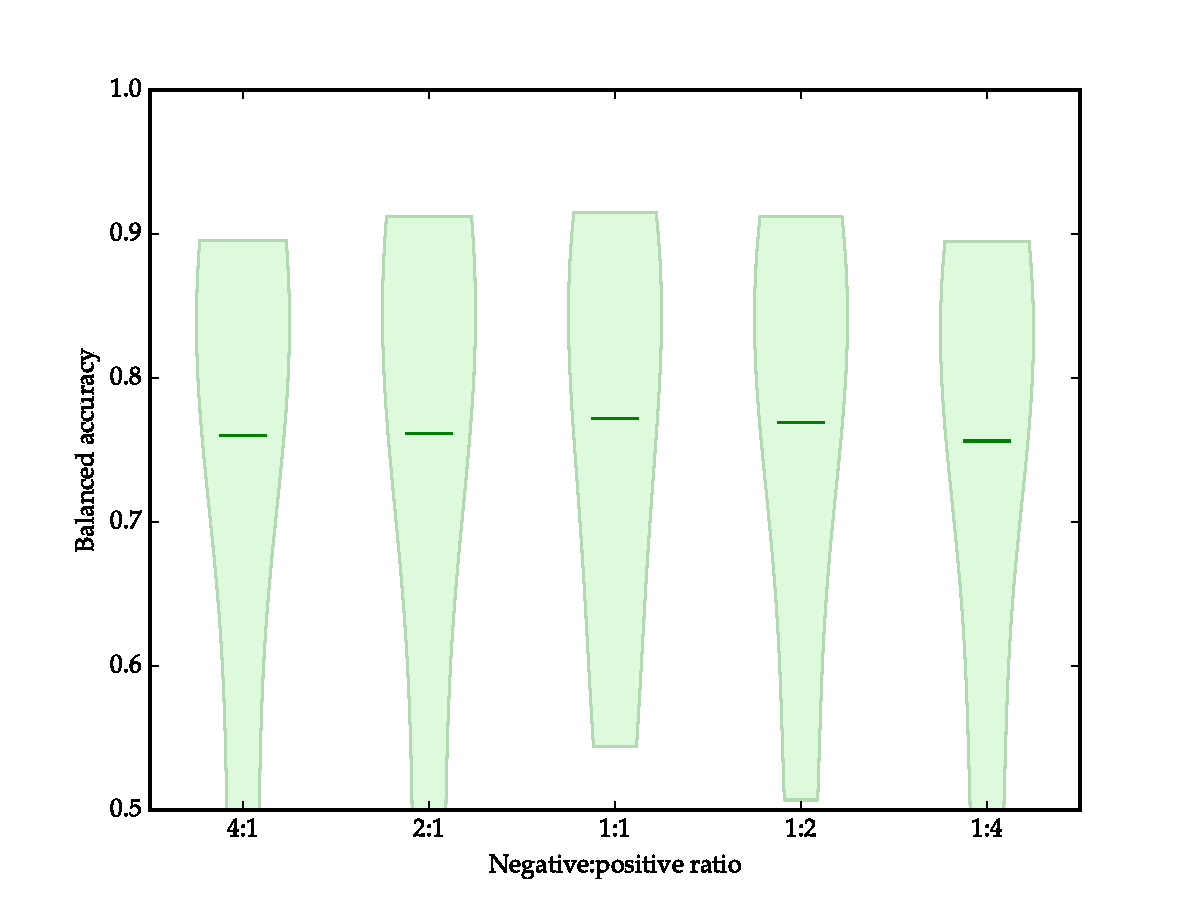
\includegraphics[width=\textwidth]
                    {images/experiments/raykar_class_balance_ba}
                \caption{Performance of the \citeauthor{raykar10} classifier on a
                    simulated labelling problem with different class imbalance.}
                \label{fig:raykar-class-balance-ba}
            \end{figure}

            \begin{figure}[!ht]
                \centering
                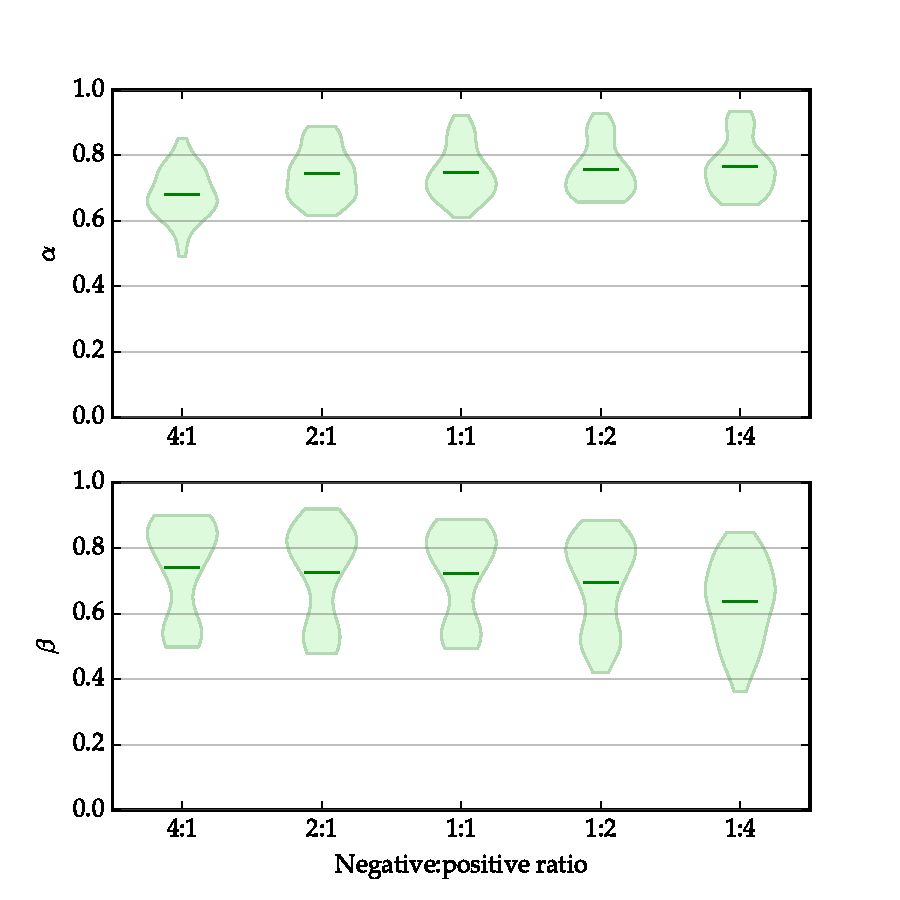
\includegraphics[width=\textwidth]
                    {images/experiments/raykar_class_balance}
                \caption{Output $\alpha$ and $\beta$ values of the
                    \citeauthor{raykar10} classifier on a simulated labelling
                    problem with different class imbalance.}
                \label{fig:raykar-class-balance-ab}
            \end{figure}

            The classifier performs well when many examples are positive, but
            performance is considerably reduced when there are more negative
            examples than positive examples. In these situations, the algorithm
            considerably underestimates $\alpha$, which may lead to ``mistrust'' of
            the crowd and hence reduce the balanced accuracy. The reason for the
            underestimation of $\alpha$ is unknown. Since we would expect the
            algorithm to perform identically under relabelling $0 \leftrightarrow
            1$, this may indicate a problem with the implementation.

        \subsubsection{The Effect of Label Noise}

            The final experiment was to determine the effect of label noise on the
            performance and output of the algorithm. 10 labellers were simulated
            with $\alpha$ ranging from $0.2$ to $1.0$ and $\beta$ fixed at $1.0$. A
            dataset was generated as for the previous experiment (but with balanced
            classes), the labellers were tasked with labelling this dataset, and the
            labels were used to train the algorithm. The balanced accuracy and
            $\alpha$ values were recorded. This experiment was repeated $5$ times,
            and repeated again with $\beta$ replacing $\alpha$. The results are
            shown in Figure

            \begin{figure}[!ht]
                \centering
                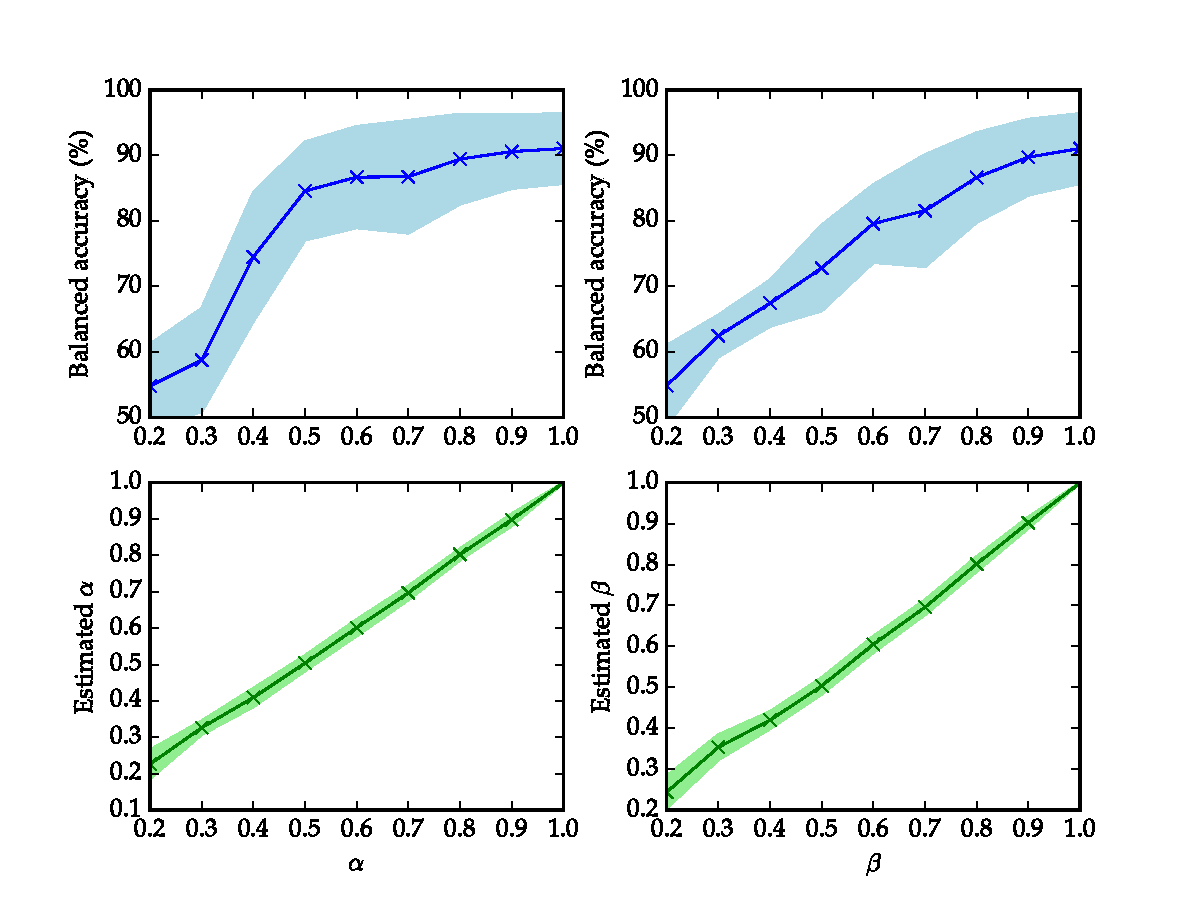
\includegraphics[width=\textwidth]{images/experiments/raykar_noise}
                \caption{Output $\alpha$, $\beta$, and balanced accuracy of the
                    \citeauthor{raykar10} classifier on a simulated labelling
                    problem with different amounts of label noise. ``Estimated
                    $\alpha$'' refers to the value of $\alpha$ output by the
                    algorithm, and $\alpha$ refers to the groundtruth. Filled areas
                    represent the standard deviation of multiple measurements.}
                \label{fig:raykar-noise}
            \end{figure}

            As expected, the balanced accuracy increases as label noise decreases.
            The output $\alpha$ and $\beta$ closely match the true values.

    \subsection{Yan et al. Model}
    \label{sec:yan}

        \todo{Clear this up with respect to the above examples.}

        \citet{yan10} propose modelling the $t$th labeller by a Bernoulli distribution of a data-dependent function $\eta_t(\vec x)$, parametrised as a logistic regression function $\eta_t(\vec x) = \sigma(\vec \omega_t^T \vec x + \gamma_t)$. The labeller model is thus
        \begin{equation*}
            p(y_t \mid \vec x, z, \vec \omega_t, \gamma_t) = \eta_t(\vec x)^{1 - |y_t - z|} (1 - \eta_t(\vec x))^{|y_t - z|}.
        \end{equation*}
        For ease of notation, let $\Omega = (\vec \omega_1^T, \dots, \vec \omega_T^T)$ and let $\vec \gamma = (\gamma_1, \dots, \gamma_T)$. This model can be obtained from the \citeauthor{raykar10} model by requiring $\alpha_t = \beta_t = \eta_t(\vec x)$ and allowing these parameters be data-dependent.

        As with \citeauthor{raykar10}, the classification model can be any classifier and \citeauthor{yan10} choose to use logistic regression (Equation \ref{eq:raykar-logreg}). The parameters $\vec \theta = \{\Omega, \vec \gamma, \vec w\}$ can be found by maximising the likelihood with expectation-maximisation. Under the assumptions that examples are independently sampled and that the labellers are independent, the likelihood is given by
        \begin{align*}
            p(\mathcal D \mid \vec \theta) &= \prod_{i = 1}^N \prod_{t = 1}^T p(y_{t, i} \mid \vec x_i, \vec w, \Omega, \vec \gamma)\\ &= \prod_{i = 1}^N \prod_{t = 1}^T \sum_{z = 0}^1 p(y_t \mid \vec x_i, z, \vec \omega_t, \gamma_t) p(z \mid \vec x_i, \vec w).
        \end{align*}
        The expectation steps requires us to compute
        \[
            \mu_i \propto \prod_{t = 1}^{T} p(y_{t, i} \mid \vec x_i, z_i = 1, \vec \omega_t, \gamma_t) p(z_i = 1 \mid \vec x_i, \vec w).
        \]
        The maximisation step requires us to maximise
        \begin{equation*}
            \sum_{i = 1}^N \sum_{t = 1}^T \sum_{z_i = 0}^1 p(z_i \mid \vec x_i, \vec w) (\log p(y_{t, i} \mid \vec x_i, z, \vec \omega_t, \gamma_t) + \log p(z \mid \vec x_i, \vec w))
        \end{equation*}
        with respect to $\vec w, \Omega,$ and $\vec \gamma$, where $p(z_i \mid \vec x_i, \vec w)$ is fixed to use the previous value of $\vec w$.